\textcolor{green}{Je suis à moitié en freestyle, à moitié en train de traduire le texte, donc il y aura sans doute beaucoup à corriger. (Julien Monfils)}

\section{Gudgeon pin \textcolor{red}{J'ai pas la traduction}}
\textcolor{red}{TODO, j'ai pas compris}

%J'ai skip 12.5 "Journal bearing load considerations" car la section n'est pas complète dans le pdf des extraits.

\section{Propriétés du matériau souhaitées pour la fabrication du bloc-moteur}
On souhaite que le matériau utilisé ai les propriétés suivantes :
\begin{itemize}
    \item Il doit être relativement peu cher
    \item Il doit pouvoir être moulé
    \item Il doit être facilement usiné
    \item Il doit être assez résistant, autant en torsion qu'en \textcolor{red}{bending => pliage ? Flambage ? Je ne trouve pas de traduction}
    \item Il doit être résistant à l'abrasion et à la corrosion
    \item Il doit avoir une dillatation thermique faible \textcolor{red}{Pas sûr de la traduction}
    \item Il doit avoir une conductivité thermique élevée
    \item Il être assez résistant à hautes températures
    \item Il doit avoir une densité relativement faible
\end{itemize}
\\

On remarque que la fonte correspond à la plus part des critères. Néanmoins, la fonte a une conductivité thermique très faible. C'est pourquoi on peut également utiliser un alliage d'aluminium léger. Il faut cependant faire attention, l'alliage d'aluminium est moins résistant à l'usure que la fonte, c'est pourquoi il faut augmenter la section du moulage \textcolor{red}{"and additional support ribs", je ne sais pas comment le traduire}. Ce qui augmente considérablement la masse du bloc-moteur en alliage.\\
De manière générale, un bloc en fonte a un masse deux fois plus élevée que celle d'un bloc en alliage d'aluminium léger.

\section{Le piston}
\begin{figure}[H]
    \centering
    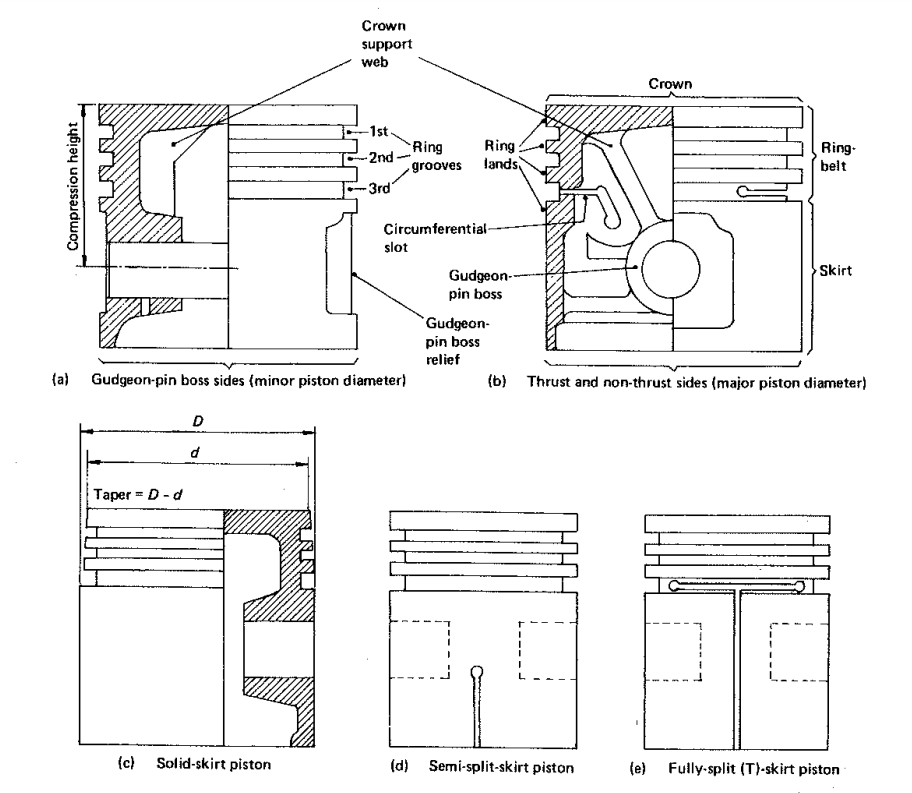
\includegraphics[width = 15cm]{Images/ImagesICE/PistonNomenclature.png}
    \caption{Fluctuation de la masse volumique en fonction du volume de l'élément \protect \footnotemark}
    \label{fig:fluctuationsVER}
\end{figure}
\footnotetext{Vehicle and engine technology, Heisler Heinz}

\textcolor{red}{TODO}